% mn2esample.tex
%
% v2.1 released 22nd May 2002 (G. Hutton)
%
% The mnsample.tex file has been amended to highlight
% the proper use of LaTeX2e code with the class file
% and using natbib cross-referencing. These changes
% do not reflect the original paper by A. V. Raveendran.
%
% Previous versions of this sample document were
% compatible with the LaTeX 2.09 style file mn.sty
% v1.2 released 5th September 1994 (M. Reed)
% v1.1 released 18th July 1994
% v1.0 released 28th January 1994

\documentclass[useAMS,usenatbib]{mn2e}
\usepackage{graphicx}
\usepackage{aas_macros}

% If your system does not have the AMS fonts version 2.0 installed, then
% remove the useAMS option.
%
% useAMS allows you to obtain upright Greek characters.
% e.g. \umu, \upi etc.  See the section on "Upright Greek characters" in
% this guide for further information.
%
% If you are using AMS 2.0 fonts, bold math letters/symbols are available
% at a larger range of sizes for NFSS release 1 and 2 (using \boldmath or
% preferably \bmath).
%
% The usenatbib command allows the use of Patrick Daly's natbib.sty for
% cross-referencing.
%
% If you wish to typeset the paper in Times font (if you do not have the
% PostScript Type 1 Computer Modern fonts you will need to do this to get
% smoother fonts in a PDF file) then uncomment the next line
% \usepackage{Times}

%%%%% AUTHORS - PLACE YOUR OWN MACROS HERE %%%%%


%%%%%%%%%%%%%%%%%%%%%%%%%%%%%%%%%%%%%%%%%%%%%%%%

\title[Statistical uncertainties in nebular abundances]{Understanding and reducing statistical uncertainties in nebular abundance determinations} %have to be the same?
\author[R. Wesson et al.]{R. Wesson$^{1,2}$, D.J. Stock$^{1,3}$ \& P. Scicluna$^{1,4}$\\
$^1$Department of Physics and Astronomy, University College London, Gower Street, London WC1E 6BT, UK\\
$^2$European Southern Observatory, Alonso de C\'ordova 3107, Casilla 19001, Santiago, Chile\\
$^3$Department of Physics and Astronomy, University of Western Ontario, London, Ontario, Canada, N6K 3K7\\
$^4$European Southern Observatory, Karl-Schwarzschildstr. 2, 85748 Garching, Germany\\ 
}


\begin{document}

\date{}

\pagerange{\pageref{firstpage}--\pageref{lastpage}} \pubyear{2002}

\maketitle

\label{firstpage}

\begin{abstract}
Whenever observations are compared to theories, an estimate of the uncertainties associated with the observations is vital if the comparison is to be meaningful.  However, many or even most determinations of temperatures, densities and abundances in photoionised nebulae do not quote the associated uncertainty.  Those that do typically propagate the uncertainties using analytical techniques which rely on assumptions that generally do not hold.

Motivated by this issue, we have developed NEAT (Nebular Empirical Analysis Tool), a new code for calculating chemical abundances in photoionised nebulae.  The code carries out a standard analysis of lists of emission lines using long-established techniques to estimate the amount of interstellar extinction, calculate representative temperatures and densities, compute ionic abundances from both collisionally excited lines and recombination lines, and finally to estimate total elemental abundances using an ionisation correction scheme.  NEAT uses a Monte Carlo technique to robustly propagate uncertainties from line flux measurements through to the derived abundances.

We show that for typical observational data, this approach is superior to analytic estimates of uncertainties.  NEAT also accounts for the effect of upward biasing on measurements of lines with low signal to noise, allowing us to accurately determine the effect of this bias on abundance determinations.  We find that the effect can result in significant over-estimates of heavy element abundances derived from weak lines, and that taking it into account improves the precision of these abundance determinations.  Finally, we investigate the effect of possible uncertainties in R, the ratio of selective to total extinction, on abundance determinations.  We find that the uncertainty due to this parameter is negligible compared to the statistical uncertainties due to typical line flux measurement uncertainties.

\end{abstract}

\begin{keywords}
ISM: abundances -- atomic processes -- methods: statistical
\end{keywords}

\section{Introduction}

Abundance determinations from photoionised nebulae play crucial roles in a variety of astrophysical contexts. Nebulae around evolved stars, e.g. Planetary Nebulae (PNe) or Wolf-Rayet (WR) ejecta nebulae provide constraints on theories of stellar nucleosynthesis and evolution (e.g. \citealt{2009ApJ...690.1130K};  \citealt{2011arXiv1110.1186M}; \citealt{1992A&A...264..105M}; \citealt{2011MNRAS.tmp.1754S}). Such data is invaluable as constraints on stellar yields; the \textit{inputs} of galactic chemical evolution models. While Galactic and extragalactic H~{\sc ii} regions provide insights into the current composition of the ISM and therefore are vital constraints for the \textit{output} of galactic chemical evolution models (e.g. \citealt{1997nceg.book.....P}; \citealt{2003ceg..book.....M}).

Such studies have a very long history \citep{1864RSPT..154..437H} \textbf{(is this gratuitously ancient enough?)}, but some major questions remain unanswered.  One long standing issue is the sometimes sizable discrepancy between abundances derived from collisionally excited lines (CELs) and those derived from recombination lines (RLs) (\citealt{2005MNRAS.362..424W}; \citet{2006MNRAS.368.1959L}; \citealt{2007ApJ...670..457G}; \citealt{2008MNRAS.386...22T}).

A meaningful comparison of observations with models is only possible if the uncertainties on the observations can be meaningfully estimated.  However, such a meaningful estimate is not trivial to determine.  The final uncertainty will be due to both statistical uncertainty (ultimately deriving from the inherent uncertainty on the original line flux measurements) and systematic uncertainty (for example, the choice of reddening law or atomic data set).  Sources of systematic uncertainty may be unknown and even unquantifiable.

In this paper we present a new code for calculating chemical abundances in photoionised nebulae, which can also robustly estimate statistical uncertainties using a Monte Carlo approach, so called because of its reliance on probabilities.  This method is inherently superior to analytic methods of uncertainty propagation. and can easily account for the effect of non-Gaussian flux uncertainties, such as those found by \citet{1994A&A...287..676R} in the case of flux measurements with low signal-to-noise ratios.

We use our code to reanalyse several published line lists for which uncertainties are available, and we show firstly that analytic methods can significantly underestimate the true uncertainties on derived quantities.  Typically, uncertainties on derived abundances are better characterised by log-normal distributions than by normal distributions, with most quantities being potentially more subject to upward bias than to downward bias.  In some cases, bimodal probability distributions emerge.

Secondly, as the Monte Carlo approach can trivially handle any quantifiable distribution of line flux uncertainties, we have designed the code to account for the well known upward bias in measurements of weak lines, and associated log-normal distribution of measurement uncertainties (\citet{1994A&A...287..676R}).  The bias is well known but its actual effect on abundance determinations has not previously been quantified.  We show, as expected, that abundances determined from weak lines are systematically overestimated.  Moreover, we show that accounting for the effect leads to a significant improvement in the precision of abundance determinations from weak lines.

Finally, we investigate the effect of an assumed statistical uncertainty in R, the ratio of selective to total extinction.  We show that the extra uncertainty introduced into abundance determinations by taking this parameter to be 3.1 $\pm$ 0.15 instead of a fixed value of 3.1 is small compared to the uncertainties arising from line flux measurements, even when the extinction is quite large and the line fluxes are well measured.

The words ``uncertainty" and ``error" are often used synonymously.  In this article we maintain a distinction in meaning between the terms: ``uncertainty" refers to the limiting accuracy of the knowledge of a quantity, while ``error" refers to an actual mistake.

\section{Statistical uncertainties}

Uncertainties in observed quantities can be propagated into the uncertainty on derived parameters in a number of different ways, the two most common of which are the traditional analytical technique based on systems of partial derivatives and simplifying assumptions that allow one to apply Taylor expansions, and the `Monte Carlo' method which is a brute-force iterative method that exploits the wealth of computational power now readily available by building on knowledge of the uncertainty in the original observations.

The analytical approach is as follows: if one has measured a quantity $x$ with some uncertainty $\sigma x$, and wishes to calculate the uncertainty in a quantity $F$ given that $F = f(x)$, then the uncertainty on $F$ can be computed via the relation 

\begin{equation}
  \frac{\sigma F}{\sigma x} \simeq \frac{\partial f}{\partial x}
\end{equation}

However, in general one may not be able to compute this partial differential exactly, and in these cases, provided that

\begin{equation}
  \frac{\partial f}{\partial x}|_{x=x_1} \ll f(x_1)
\end{equation}

it is possible to use a first order Taylor expansion to approximate this derivative.  If one had a third value, $H = h(f, g)$ where $f$ and $g$ are both functions of other variables and are statistically independent of one another, it would be necessary to find the total derivative $dH$ such that

\begin{equation}
dh^2 = \left(\frac{\partial h}{\partial f}\right)^2df^2 + \left(\frac{\partial h}{\partial g}\right)^2dg^2
\end{equation}

and it thus follows that

\begin{equation}
\sigma^2_H = \left(\frac{\partial h}{\partial f}\sigma f\right)^2 + \left(\frac{\partial h}{\partial g}\sigma g\right)^2
\end{equation}

This expression can be generalised to any number of variables, and gives rise to the usual quadrature formulae for many simple functions of $x$.  We highlight three key aspects of this approach:

\begin{enumerate}
  \item Given the number of formulae through which the original line flux data must be put before an abundance can be determined, and the wide variety of functions applied, the equations necessary to propagate uncertainties in this way can become extremely complex;
  \item the approach implicitly assumes that all the input and output uncertainties at each step are normally distributed;
  \item the Taylor expansion requires that the uncertainties be small relative to the quantities.
\end{enumerate}

The first point is a matter of convenience but none the less one which discourages many authors from even attempting to propagate uncertainties all the way into the final quantities.  The second and third points are clearly violated in many or most real astrophysical observations, by virtue of which the uncertainties estimated using analytical techniques are liable not to reflect the true uncertainties.

The Monte Carlo method, on the other hand, exploits the fact that if an observation of a quantity is drawn from a distribution $X$, with mean $x$ and variance $\sigma_x$ , and if one knows (or can make sensible assumptions about) the shape of this distribution, then a random-number generator can be used to repeatedly draw values from X, creating a random sample from it. Using the above example of $F = f (x)$, if one wanted to examine the uncertainty in F, the operation f(x) could be performed upon every value in the aforementioned sample to produce a sample of the distribution from which F is drawn, which can then be parameterised to estimate the type, mean and standard deviation of this distribution. This process can be repeated ad infinitum for any number or combination of functions of F, x, or any other variable derived in the same way to propagate the uncertainties on the quantities, irrespective of the size of the uncertainties and any statistical interdependence of the variables.  This approach thus has the following advantages over the analytical approach:

\begin{enumerate}
  \item It is inherently very simple;
  \item it requires no assumption about the particular distribution of uncertainties at any stage;
  \item it does not require relative uncertainties to be small
\end{enumerate}

The Monte Carlo approach is thus inherently robust when applied to real astrophysical data, in a way that the analytical approach is not.  The only limitation is then the time taken to run the calculation enough times to sample well the statistics of the output distributions.

\section{NEAT: Nebular empirical abundance tool}

We have developed a new code, NEAT (Nebular Empirical Analysis Tool), to quickly carry out a thorough analysis of emission line spectra, and to propagate statistical uncertainties using the Monte Carlo technique described above.  In this section we describe the code and how it works.

\subsection{Input}

{\sc neat} incorporates elements of several previous codes, most importantly the {\sc equib} code, also developed at UCL, for solving the equations of statistical equilibrium in multi-level atoms.  All the source code, documentation, atomic data and example line lists are freely available at \texttt{https://github.com/rwesson/NEAT}.  The code is designed to be as simple as possible from the user's perspective, and our aim is that the user should be able to simply pass the code a line list and get out abundances determined robustly.  The code requires no external libraries and should compile without problems on any Unix system.  We have also verified that it compiles and runs on Windows systems, should the user be restricted to such an OS.

Hydrogen recombination data from \citet{1995MNRAS.272...41S} is used throughout.  All atomic data for heavier elements is stored externally in plain text files, so that the user can easily change the atomic data being used without needing to recompile the code.  We provide three sets of atomic data for collisionally excited lines with the code - a compilation from a variety of sources compiled on an ad hoc basis, CHIANTI 5.2 \citep{2006ApJS..162..261L}, and CHIANTI 6.0 \citep{2009A&A...498..915D,}.  In all the analyses presented in this paper, we used atomic data from CHIANTI 5.2, with the exception of data for O$^{2+}$ for which a documented error exists in the CHIANTI 5.2 data \citep{2009MNRAS.397..903K}, and S$^{3+}$, which we believe is affected by a similar error.  Data for these two ions was instead taken from (cite) and (cite) respectively.  For recombination lines, we use data from the sources given in Table~\ref{RL_atomic_data}.

\begin{table}
\begin{tabular}{ll}
\hline
Ion & Recomination data source \\
\hline
C$^{2+}$ & \\
C$^{3+}$ & \\
N$^{2+}$ & \\
N$^{3+}$ & \\
O$^{2+}$ & \\
Ne$^{2+}$& \\
\hline
\end{tabular}
\label{RL_atomic_data}
\caption{Atomic data used in {\sc NEAT} for recombination lines}
\end{table}

{\sc neat} requires as input a plain text list of rest wavelengths, line fluxes, and uncertainties.  The user can then select the number of iterations of the code to run.  If the number of iterations is one, the code performs a standard empirical analysis on the line list, as described below, and does not calculate any uncertainties.  If the number of iterations is more than one, then the code first randomises the line list, as described below.  The standard analysis is then carried out on the randomised line list.

By randomising and analysing the line list many times, it is possible to build up an accurate picture of the true distribution of statistical uncertainties associated with the chemical abundances and empirical diagnostics resulting from the line flux uncertainties. {\sc NEAT} collates all of the results from each iteration, and generates histograms showing visually the uncertainty distributions on the output parameters.

\subsubsection{Line flux randomisation}
\label{randomising}

The code randomises the line fluxes by assuming that they come from one of three distributions, depending on the measured signal to noise.  The three cases are:

{\bf SNR$>$6.0: } the line flux is assumed to be drawn from a Gaussian distribution.  In this case, if the given line flux measurement is $F$ and the given measurement uncertainty is $\sigma$, then in each iteration of the code the line flux is calculated using

\begin{equation}
F_i = F + R\times\sigma
\end{equation}

where R is a random number drawn from a Gaussian distribution with a mean of zero and a standard deviation of unity.

{\bf 1.0$<$SNR$<$6.0: } \citet[][hereafter RP94]{1994A&A...287..676R} observed that measurements of weak lines (SNR$<$6) are strongly biased upwards, and the uncertainty on such lines cannot be well represented by a normal distribution.  We refer to this effect henceforth as the RP effect.  Taking the RP94 effect into account is straightforward with a Monte Carlo approach, requiring only that a log-normal distribution with appropriate mean and standard deviation is used for weak lines, instead of the normal distribution used for strong lines.

For lines with F/$\sigma < $6, we randomise the line fluxes using the following procedure: we first determine the log-normal distribution appropriate to the measured signal-to-noise ratio using the following equations, which are derived from fits to the numbers in Table 6 of RP94:

\begin{equation}
\mu = \frac{0.0765957}{snr^2} + \frac{1.86037}{snr} - 0.309695
\end{equation}

\begin{equation}
\sigma = \frac{-1.11329}{snr^3} + \frac{1.8542}{snr^2} - \frac{0.288222}{snr} + 0.18018
\end{equation}

Then, the line flux is found using the following equation:

\begin{equation}
F_i = \frac{F}{e^{(R\times\sigma + \mu)}}
\end{equation}

where R is a random number from a gaussian distribution as before.  The result of this procedure is that weaker lines are drawn from log-normal distributions that peak below the observed value, with the effect increasing as SNR decreases.  The statistical behaviour is as described by RP94.

{\bf SNR$<$1.0: } If the quoted uncertainty is larger than the acual line flux, the code assumes that the quote flux represents a 5$\sigma$ upper limit, and thus draws the randomized line flux from a folded gaussian distribution, with $\mu$=0 and $\sigma$=0.2$\times$F.  The line flux is given by

\begin{equation}
F_i = abs(R)\times0.2F
\end{equation}

Figure~\ref{distributions} shows the various possibilities that arise depending on the measured SNR.  The distributions plotted are from 10$^6$ runs of NEAT in which 7 artificial line fluxes were randomized.  Each of the lines had a measured flux of 10.0, and the quoted uncertainties represented SNRs of 1.0, 2.0, 3.0, 4.0, 5.0, 6.0 and 8.0.  The figures shows how the normal distribution appropriate at high SNR is replaced by a log-normal distribution increasingly skewed towards lower values as SNR decreases.

\begin{figure}
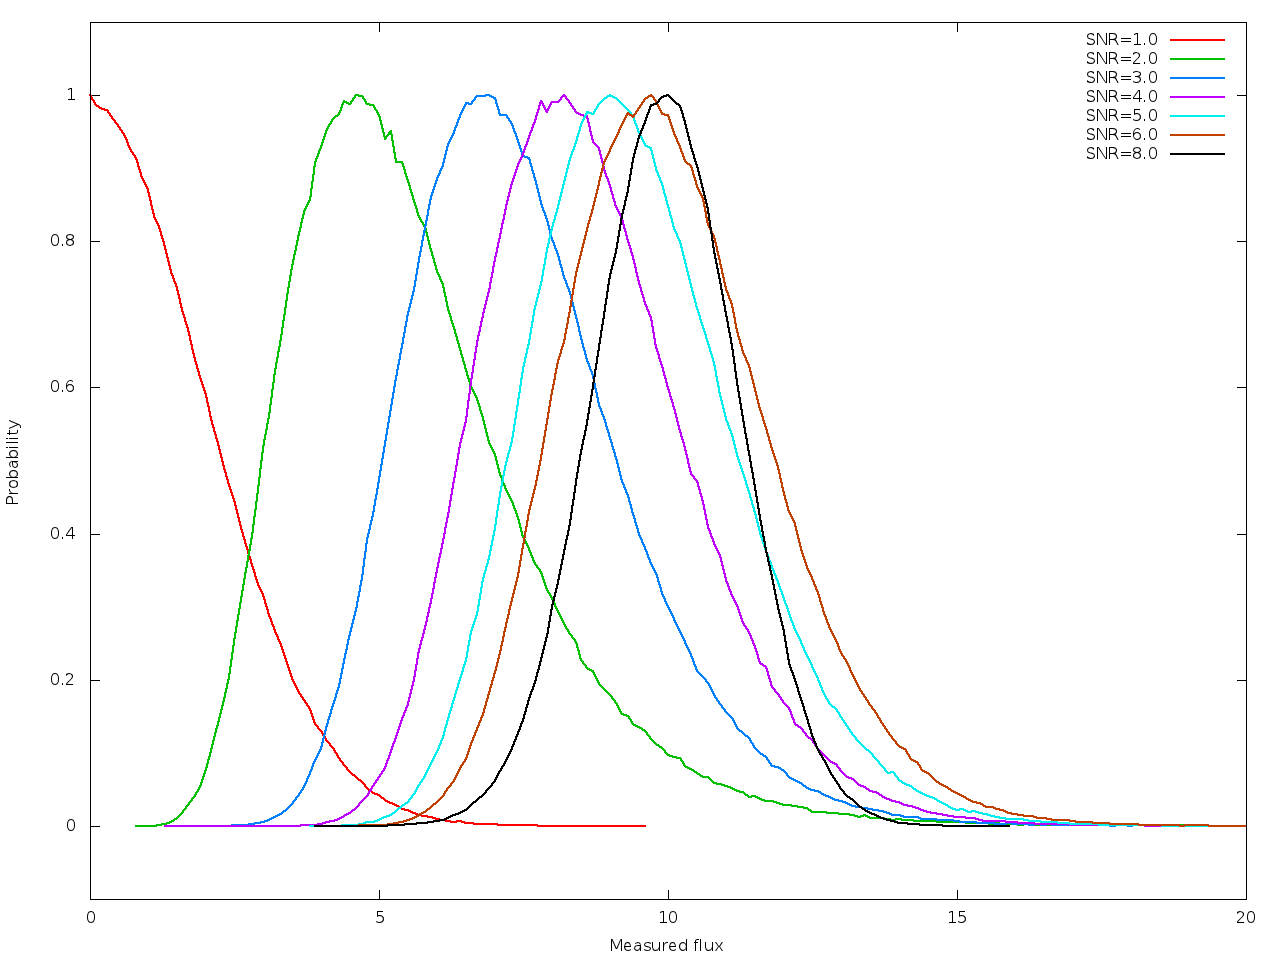
\includegraphics[width=0.47\textwidth]{figures/distributions_2.png}
\caption{The behaviour of NEAT's line flux randomization as a function of SNR, for a fixed measured flux of 10.0.  At high SNR (i.e. $>$6), normal distributions apply.  At lower SNR, the effect described by \citet{1994A&A...287..676R} results in log-normal distributions which are skewed towards lower values than the measured intensity.  If SNR$\leq$1 then the code assumes that the quoted flux is a 5$\sigma$ upper limit}
\label{distributions}
\end{figure}

\subsubsection{Random number algorithm}

This process relies on the FORTRAN pseudo-random number generator, seeded using the system clock and the time of the code's exection.  The uniformly distributed numbers thus generated are then converted into a gaussian distribution using an algorithm based on the ratio of uniforms method of \citet{Kinderman:1977:CGR:355744.355750}, available from \texttt{netlib.org}.  We tested the performance of this method by running the code 1\,000\,000 times, and plotting the distribution of fluxes obtained for an arbitrarily selected line.  We then fitted a gaussian function to this distribution.  We found that the recovered mean was within 0.008\% of the specified value, while the recovered standard deviation was within 0.13\% of the specified value.  Figure~\ref{gaussiantest} shows the histogram of generated values with the required gaussian distribution overplotted.  We thus consider that the random number generator in the code provides a reliably random Gaussian distribution.

\begin{figure}
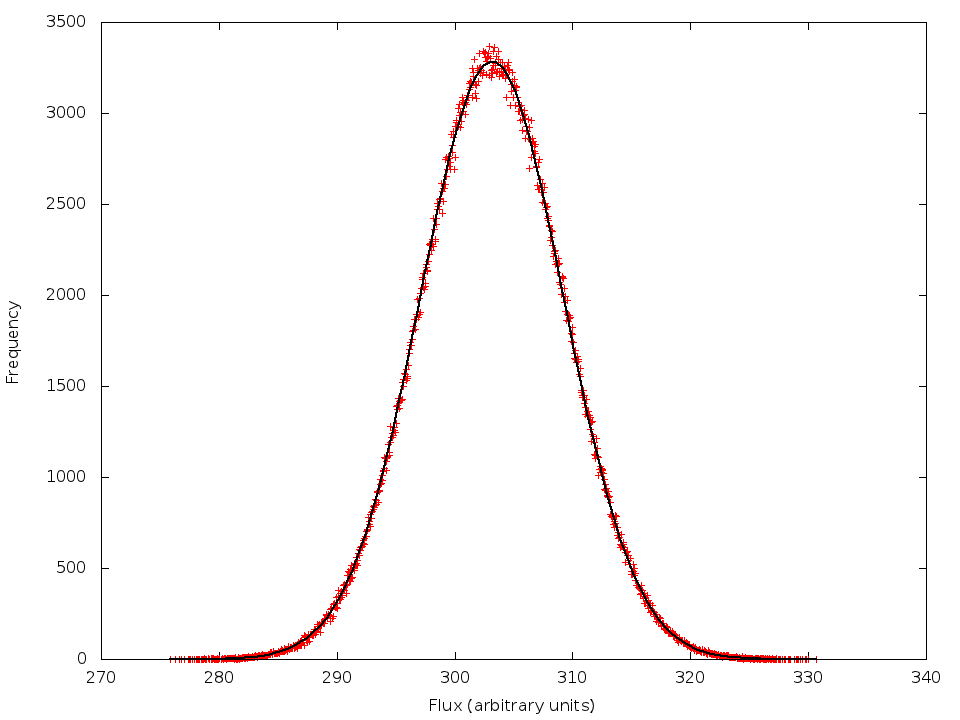
\includegraphics[width=0.47\textwidth]{figures/gaussian_test.png}
\caption{A distribution of values produced by 1\,000\,000 runs of the random number generator, with the target gaussian distribution overplotted.}
\label{gaussiantest}
\end{figure}

\subsubsection{Sampling uncertainty}

The Monte Carlo approach relies on carrying out the analysis enough times to adequately sample the probability distributions of the derived quantities.  To determine what number of iterations suffices for this purpose, we ran the code 1,000,000 times, using emission line fluxes measured for IC1747 by \citet{2005MNRAS.362..424W}.  We then considered subsets of the output from this run.

To quantify the sampling uncertainty, we fitted a gaussian to the observed probability distribution of the measured [O~{\sc iii}] temperatures, for each subset of iterations.  We chose this quantity as its actual uncertainty distribution should closely approximate a gaussian.  The uncertainty on the gaussian fit is thus a measure of how well the output distribution was sampled, for a given number of iterations.

In Figure~\ref{samplefigure1} we show how the uncertainty of the fitted $\mu$ and $\sigma$ vary with the total number of iterations.  We find that the precision of the fit improves indefinitely with increasing number of iterations up to the limit of our investigation.  However, we find that approximately 10,000 iterations provides a sensible trade-off - more iterations than this gives little absolute reduction in the sampling uncertainty.  We therefore carry out 10,000 iterations on each line list used in our analyses here.

\begin{figure*}
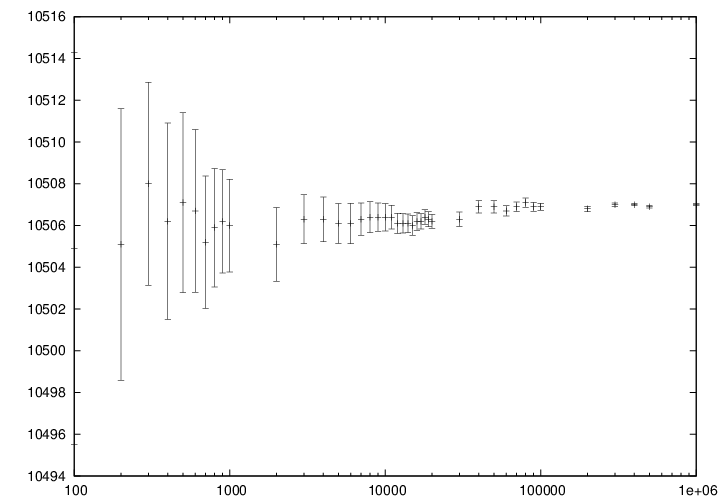
\includegraphics[width=0.48\textwidth]{figures/mulogx.png}
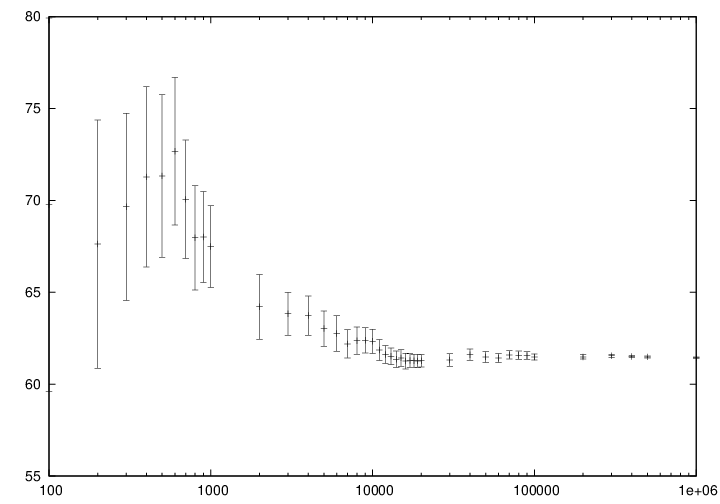
\includegraphics[width=0.48\textwidth]{figures/sigmalogx.png}
\caption{The dependence of the sampling uncertainty on the number of iterations.  Sampling uncertainty is quantified as described in the text.  10,000 iterations provides a sensible balance of acceptable processing time and sampling uncertainty.}
\label{samplefigure1}
\end{figure*}

\subsection{Interstellar extinction}

The first step of any abundance analysis is a correction for interstellar extinction.  The amount of extinction is determined by NEAT from the ratios of hydrogen Balmer lines, in an iterative procedure: the extinction is first calculated assuming intrinsic H$\alpha$, H$\beta$ and H$\gamma$ line ratios for a temperature of 10\,000\,K and a density of 1000\,cm$^{-3}$.  The line list is dereddened using the value of c(H$\beta)$ thus obtained, and temperatures and densities calcaulted as described below.  The intrinsic Balmer line ratios are then recalculated at the appropriate temperature and density, and the line list dereddened using this revised value.

The user can select the particular extinction law to be used.  Five extinction laws are currently available: the Galactic extinction curves of \citet{1983MNRAS.203..301H}, \citet{1990ApJS...72..163F} and \citet{1989ApJ...345..245C}, the Large Magellanic Cloud law of \citet{1983MNRAS.203..301H}, and the Small Magellanic Cloud law of \citet{1984A&A...132..389P}.  Adding further extinction laws would be straightforward, should the user wish to do so.

In section~\ref{extinction} we investigate the effect on derived quantities of the likely uncertainty in $R$, the ratio of selective to total extinction.

\subsection{Temperatures and densities}

Temperatures and densities are calculated using traditional collisionally excited line diagnostics.  For the purposes of subsequent abundance calculations, the nebula is divided into three ``zones", of low, medium and high excitation.  In each zone, temperatures and densities are calculated iteratively and weighted according to the reliability of each diagnostic.  Table~\ref{zonestable} shows the diagnostics used and the weighting given in each zone.

The scheme to calculate the densities is iterative, and proceeds as follows:

\begin{enumerate}
\item A temperature of 10,000K is initially assumed, and the density is then calculated from the line ratios relevant to the zone.
\item The temperature is then calculated from the temperature diagnostic line ratios, using the derived density.
\item The density is recalculated using the appropriately weighted average of the temperature diagnostics
\item The temperature is recalculated using this density.
\end{enumerate}

This iterative procedure is carried out successively for low, medium and high ionisation zones, and in each case if no diagnostics are available, the temperature and/or density will be taken to be those derived for the previous zone.

\begin{table}
\begin{tabular}{ccc}
\hline
\multicolumn{3}{c}{Low ionisation zone}\\
\hline
Diagnostic & Lines & Weight \\
~[O~{\sc ii}] density & $\lambda$3727/$\lambda$3729 & 1 \\
~[S~{\sc ii}] density & $\lambda$6717/$\lambda$6731 & 1 \\
~\\
~[N~{\sc ii}] temperature & $\frac{\lambda 6548 + \lambda 6584}{\lambda 5754}$ & 5 \\
~[S~{\sc ii}] temperature & $\frac{\lambda 6717 + \lambda 6731}{\lambda 4068 +  \lambda 4076}$ & 1 \\
~[O~{\sc ii}] temperature & $\frac{\lambda 7319,20 + \lambda 7330,31}{\lambda 3726 + \lambda 3729}$ & 1 \\
~[O~{\sc i}] temperature & $\frac{\lambda 6363 + \lambda 6300}{\lambda 5577}$ & 1 \\
~[C~{\sc i}] temperature & $\frac{\lambda 9850 + \lambda 9824}{\lambda 8727}$ & 1 \\
\hline
\multicolumn{3}{c}{Medium ionisation zone}\\
\hline
Diagnostic & Lines & Weight \\
~[Cl~{\sc iii}] density & $\lambda$5517/$\lambda$5537 & 1 \\
~[Ar~{\sc iv}] density & $\lambda$4711/$\lambda$4740 & 1 \\
~[C~{\sc iii}] density & $\lambda$1907/$\lambda$1909 & 1 \\
~[O~{\sc iii}] density & $\lambda$52$\mu$m/$\lambda$88$\mu$m & 0 \\
~[Ar~{\sc iii}] density & $\lambda$9$\mu$m/$\lambda$21.8$\mu$m & 0 \\
~[S~{\sc iii}] density & $\lambda$18.7$\mu$m/$\lambda$33.8$\mu$m & 0 \\
~[Ne~{\sc iii}] density & $\lambda$15.5$\mu$m/$\lambda$36.0$\mu$m & 0 \\
~\\
~[O~{\sc iii}] temperature & $\frac{\lambda 4959 + \lambda 5007}{\lambda 4363}$ & 4\\
~[Ar~{\sc iii}] temperature &7135 + 7751/5192 & 2\\
~[Ne~{\sc iii}] temperature & 3868 + 3967/3342 & 2\\
~[S~{\sc iii}] temperature & 9069 + 9531/6312 & 1\\
~[Ne~{\sc iii}] temperature & 3868 + 3967/15.5$\mu$m & 0\\
~[O~{\sc iii}] temperature &4959 + 5007/52 & 0\\
\hline
\multicolumn{3}{c}{High ionisation zone}\\
\hline
Diagnostic & Lines & Weight \\
~[Ne~{\sc iv}] density & 2423/2425 & 1 \\
~\\
~[Ar~{\sc v}] temperature & 6435 + 7005/4625& 1 \\
~[Ne~{\sc v}] temperature & 3426 + 3345/2975 & 1 \\
\end{tabular}
\label{zonestable}
\caption{Diagnostics used in the calculation of physical conditions.}
\end{table}

\subsection{Ionic abundances}

Ionic abundances are calculated from collisionally excited lines using the temperature and density appropriate to their ionisation potential.  Where several lines from a given ion are present, the ionic abundance adopted is found by averaging the abundances from each ion, weighting according to the observed intensity of the line.

Recombination lines are also used to derive ionic abundances for helium and heavier elements.  In deep spectra, many more recombination lines may be available than collisionally excited lines.  The code first assigns IDs to each line based on their rest wavelengths, and then calculates the ionic abundance from the line intensity using the atomic data listed in Table~\ref{RL_atomic_data}.  Then, to determine the ionic abundance to adopt, it first derives an ionic abundance for each individual multiplet from the multiplet's co-added intensity, and then averages the abundances derived for each multiplet to obtain the ionic abundance used in subsequent calculations.

\subsection{Total elemental abundances}

Generally, not all ionisation stages of an ion that are actually present in a nebula will be detected, due to limited wavelength coverage and sensitivity.  Total elemental abundances must be estimated using ionisation correction schemes, which are derived from photoionisation models, or similarities in ionisation potentials, or a combination of the two.

The code currently includes the ICF scheme of \citet{1994MNRAS.271..257K}.  We plan to incorporate further ICFs, and in a forthcoming paper we will compare the magnitude of the systematic uncertainties arising from the choice of ICF with the statistical uncertainties.

\section{Comparing analytic and Monte Carlo uncertainties}

To demonstrate how traditional methods of uncertainty propagation do not properly reflect the true uncertainties on the derived chemical abundances, we present here a reanalysis using NEAT of observations of the nebula surrounding the Large Magellanic Cloud Wolf-Rayet star WR18.  These observations were presented by \citet{2011MNRAS.tmp.1754S} and analysed using an earlier version of NEAT.  In this section we calculate the abundances and uncertainties using both the current version of NEAT, which accounts for non-Gaussian line flux uncertainties, and using analytical techniques.

We chose this object as it is distant and faint, and the line measurements are thus necessarily measured with relatively low signal to noise ratios, and the effects of the assumptions in the analytical method are most apparent.  The results of this analysis are presented in Table~\ref{WR18_uncertainties_table}.

%wo objects, along with the results from a third object which was originally analysed with NEAT (WR 18).  We chose objects having very deep, moderately deep and shallow spectra.  \citet{2011MNRAS.415..181F} presented a spectrum of NGC 7009 containing approximately 1300 identified emission lines.  NGC\,6543 \citep{2004MNRAS.351.1026W} has a spectrum with about 200 emission lines measured, and WR18 \citep{2011arXiv1108.3800S} has 36 lines detected.

%Discussions of Gaussian v. non-Gaussian distributions.  Bi-modal.  ICF complications.

\section{The nature of actual uncertainties}

General comments on what typically emerges - approximately gaussian for quantities derived from simple functions of well-measured inputs, mostly lognormal for most things, sometimes crazy.

\section{The RP effect}

As discussed earlier, NEAT accounts for the RP effect, in which fluxes measured from lines with SNR$<$6 are generally overestimated, with the magnitude of the effect increasing as SNR$\to$1.  In this section we show the importance of this effect and demonstrate that flawed results will inevitably result if the effect is ignored.

To investigate the magnitude of this effect, we reanalysed two line lists - spectra of NGC\,6543, the Cat's Eye Nebula, presented by \citet{2004MNRAS.351.1026W}, and spectra of the Orion Nebula presented by \citet{2004MNRAS.355..229E}.  In both cases we ran two instances of NEAT, one in which the RP effect was ignored, and all line flux uncertainties quoted in the two papers were assumed to represent gaussian probability distributions, and the second in which the RP effect was accounted for as described in Section~\ref{randomising}.

One important and as yet unresolved issue in nebular abundance studies is the so-called abundance discrepancy problem (see for example \citet{2006IAUS..234..219L} for a recent review).  The RP effect can cause errors in the assessment of the magnitude of the discrepancy; recombination lines of heavy elements are much weaker than the collisionally excited lines of the same species, and are thus measured with lower signal to noise ratios.  In almost any real astronomical spectra, regardless of the number of lines detected, the weakest lines measured will be subject to the RP effect, and for deep spectra of photoionised nebulae, the weakest lines will almost all be recombination lines.  Thus, recombination line abundance measurements may be subject to an upward bias that collisinally excited line abundances are largely free from.

Figure~\ref{RP_figures} shows that in these two nebulae, the RP effect indeed has no effect on abundances of nitrogen, oxygen and neon derived from collisionally excited lines, but in all cases leads to an overestimate of the abundances derived from the recombination lines of these elements.  Furthermore, it turns out that properly accounting for the non-Gaussian nature of the uncertainties on weak lines leads to a significant improvement in the precision of abundances determined from them; we fit the resulting uncertainty histograms with gaussian functions, and find that accounting for the RP effect reduces the standard deviation on the measured abundances by 30-40\%.  Table~\ref{RP_numbers} summarises the mean and standard deviation of the final abundance determinations from recombination lines.

\begin{table*}
\begin{tabular}{l ll l}
Element & 10$^4 \times$ X/H (RP ignored) & 10$^4 \times$ X/H (RP included) & $\frac{\sigma (RP included)}{\sigma (RP ignored)}$ \\
\multicolumn{4}{c}{Orion}\\

N & 2.74 $\pm$ 0.16 & 2.37 $\pm$ 0.11 & 0.69 \\
O & 7.04 $\pm$ 0.63 & 6.63 $\pm$ 0.43 & 0.69 \\
Ne & 1.52 $\pm$ 0.26 & 1.20 $\pm$ 0.17 & 0.66 \\

\multicolumn{4}{c}{NGC 6543} \\

N & 6.93 $\pm$  0.56 & 5.83 $\pm$  0.37 & 0.66 \\
O & 14.94 $\pm$ 1.15 & 12.48 $\pm$ 0.74 & 0.65 \\
Ne & 4.17 $\pm$ 0.94 & 3.23 $\pm$ 0.56 & 0.60 \\

\end{tabular}
\caption{Results of heavy element abundance determinations from recombination lines, using the published line lists of \citet{2004MNRAS.351.1026W} and \citet{2004MNRAS.355..229E} for the Orion Nebula.}
\label{RP_numbers}
\end{table*}

\begin{figure*}
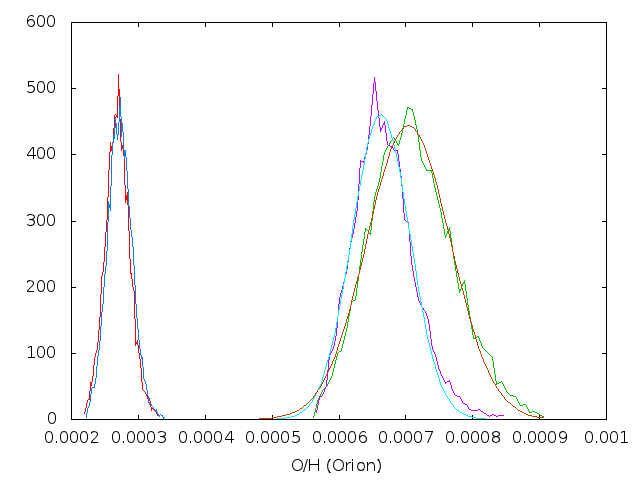
\includegraphics[width=0.48\textwidth]{figures/orion_O_rpeffect.png}
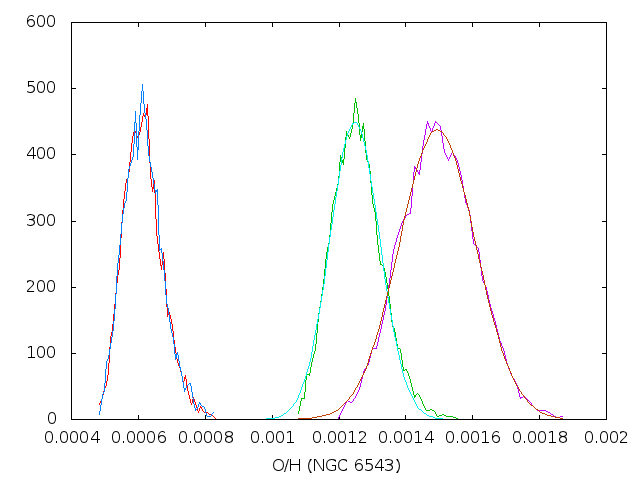
\includegraphics[width=0.48\textwidth]{figures/ngc6543_o_rpeffect.png}
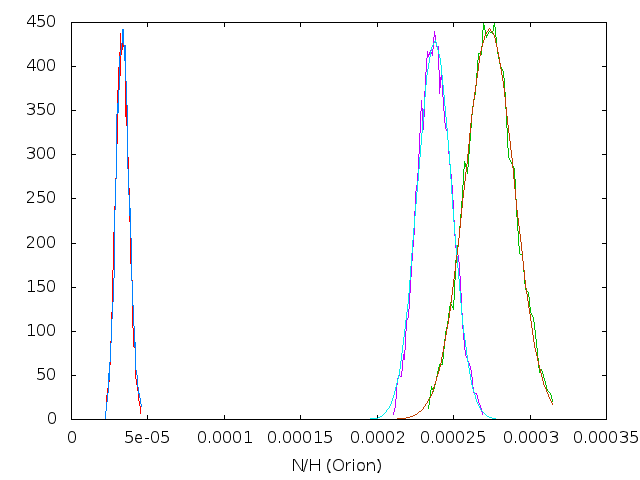
\includegraphics[width=0.48\textwidth]{figures/orion_N_rpeffect.png}
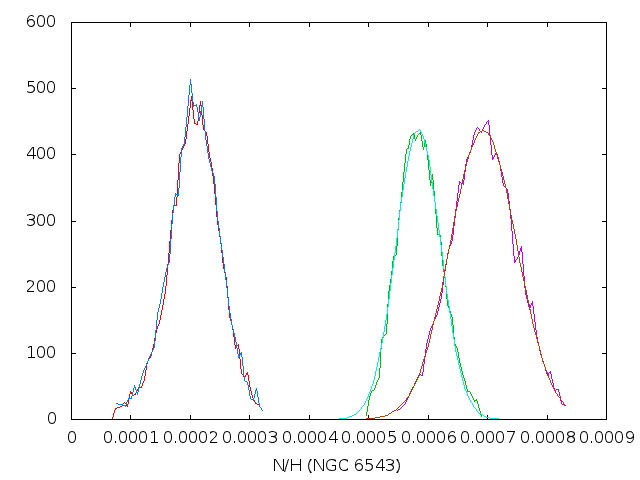
\includegraphics[width=0.48\textwidth]{figures/ngc6543_n_rpeffect.png}
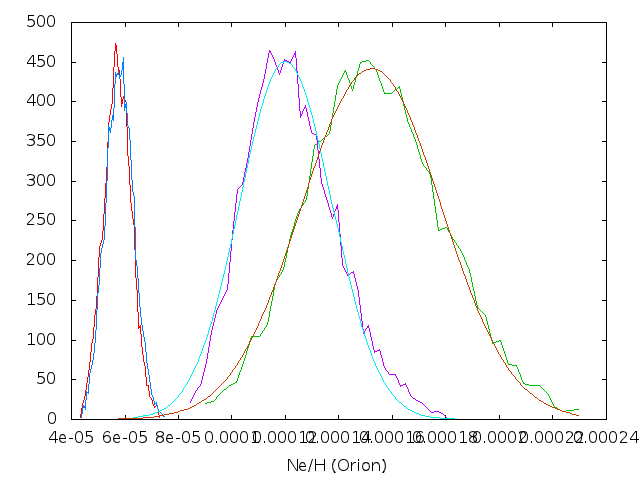
\includegraphics[width=0.48\textwidth]{figures/orion_Ne_rpeffect.png}
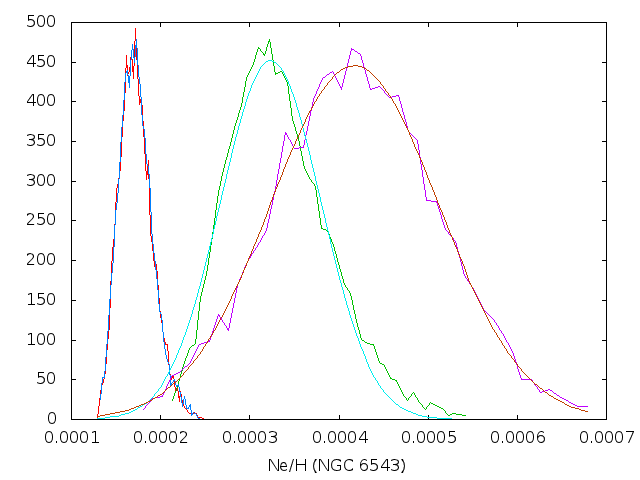
\includegraphics[width=0.48\textwidth]{figures/ngc6543_ne_rpeffect.png}
\caption{Figures comparing abundance determinations from weak lines carried out by incorrectly assuming normally distributed uncertainties with those in which weak line uncertainties are characterised following RP94}
\label{RP_figures}
\end{figure*}

In other shallower spectra, it may often be the case that the auroral lines [N~{\sc ii}] $\lambda$5754 and [O~{\sc iii}] $\lambda$4363 are measured with low enough SNR that they become subject to the RP effect.  In this case, the derived temperatures would be overestimated, and collisionally excited line abundances underestimated.  To investigate this effect, we analysed the line list of H1013, an extragalactic H~{\sc ii} region in the spiral galaxy M101, presented by \citet{2009ApJ...700..654E}.  In this nebula, the [O~{\sc iii}] line at 4363{\AA} is detected with an SNR of only 2.7.

Figure~\ref{h1013_RP_effect} shows that significant systematic uncertainties are produces when the RP effect on temperature diagnostic lines is ignored.  When the effect is neglected, we determine an [O~{\sc iii}] temperature of 7480$\pm$610\,K, in very close agreement with the value of 7370$\pm$630\,K reported by \citet{2009ApJ...700..654E}.  However, when we account for the RP effect, we find a value of 6840$\pm$390\,K.  Similarly for abundances, considering O$^{2+}$/H$^+$, we find that by neglecting the RP effect we obtain a value of 7.95$\pm$0.15 (on a logarithmic scale where N(H)=12), close to the value of 8.05$\pm$0.12 obtained by \citet{2009ApJ...700..654E}.  Accounting for the effect yields a value of 8.16$\pm$0.12.

We re-emphasise, therefore, that neglecting this effect results in incorrect abundances.  Accounting for it improves both the accuracy and precision of the abundances determined.

\begin{figure*}
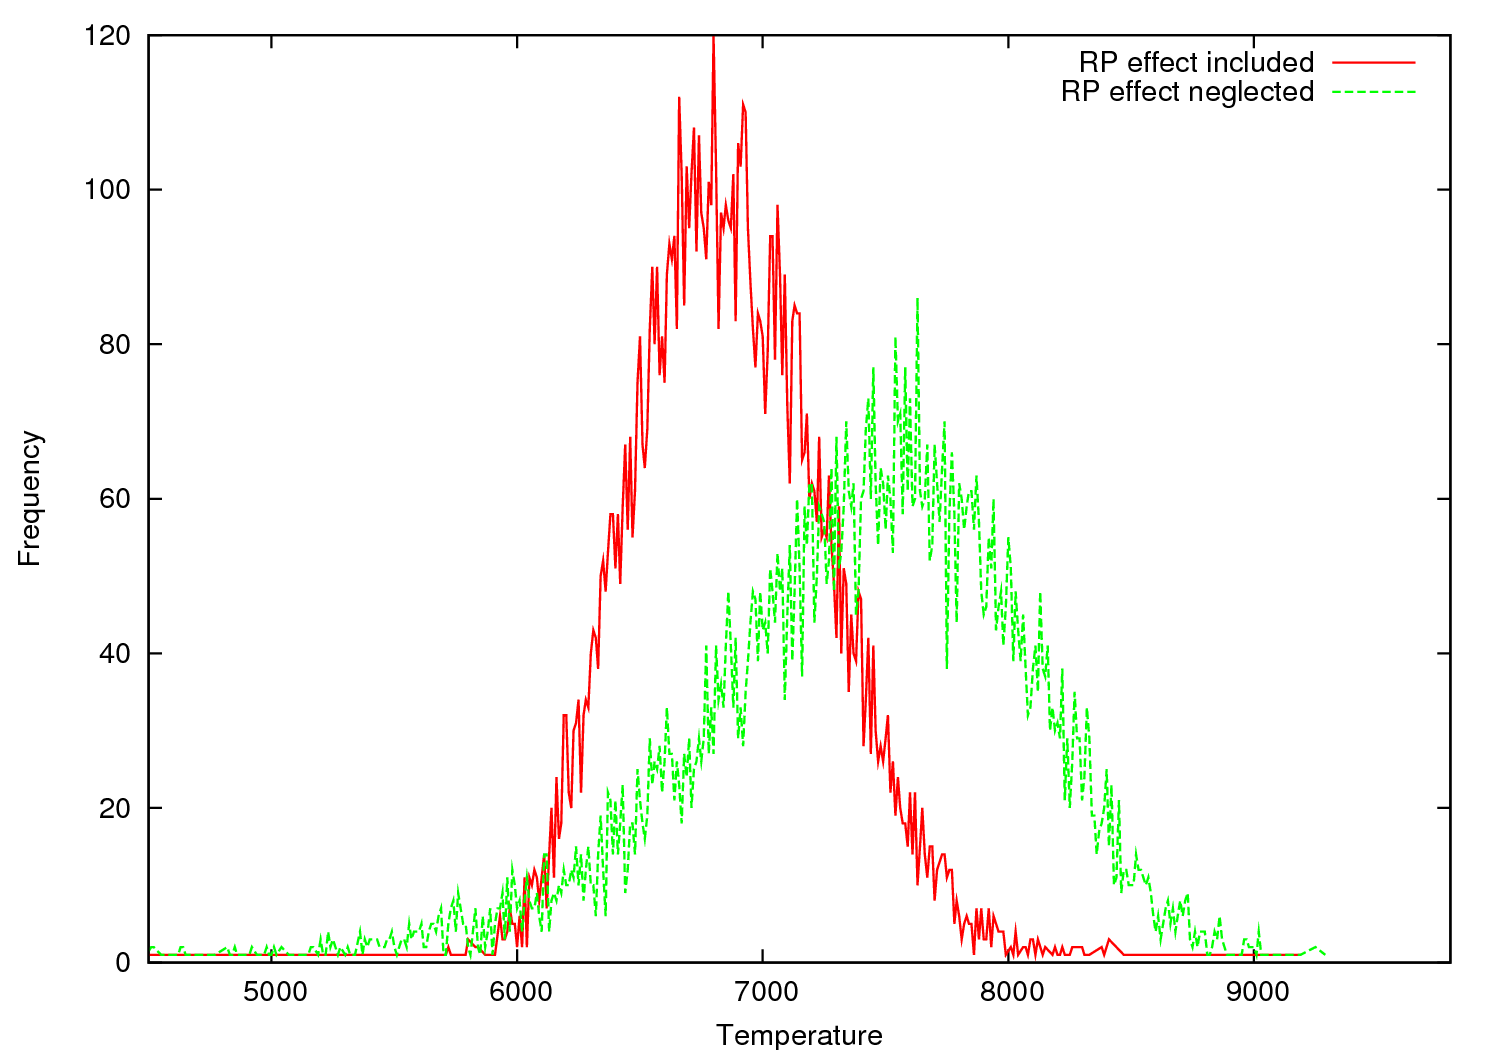
\includegraphics[width=0.48\textwidth]{figures/h1013_rp_temperature.png}
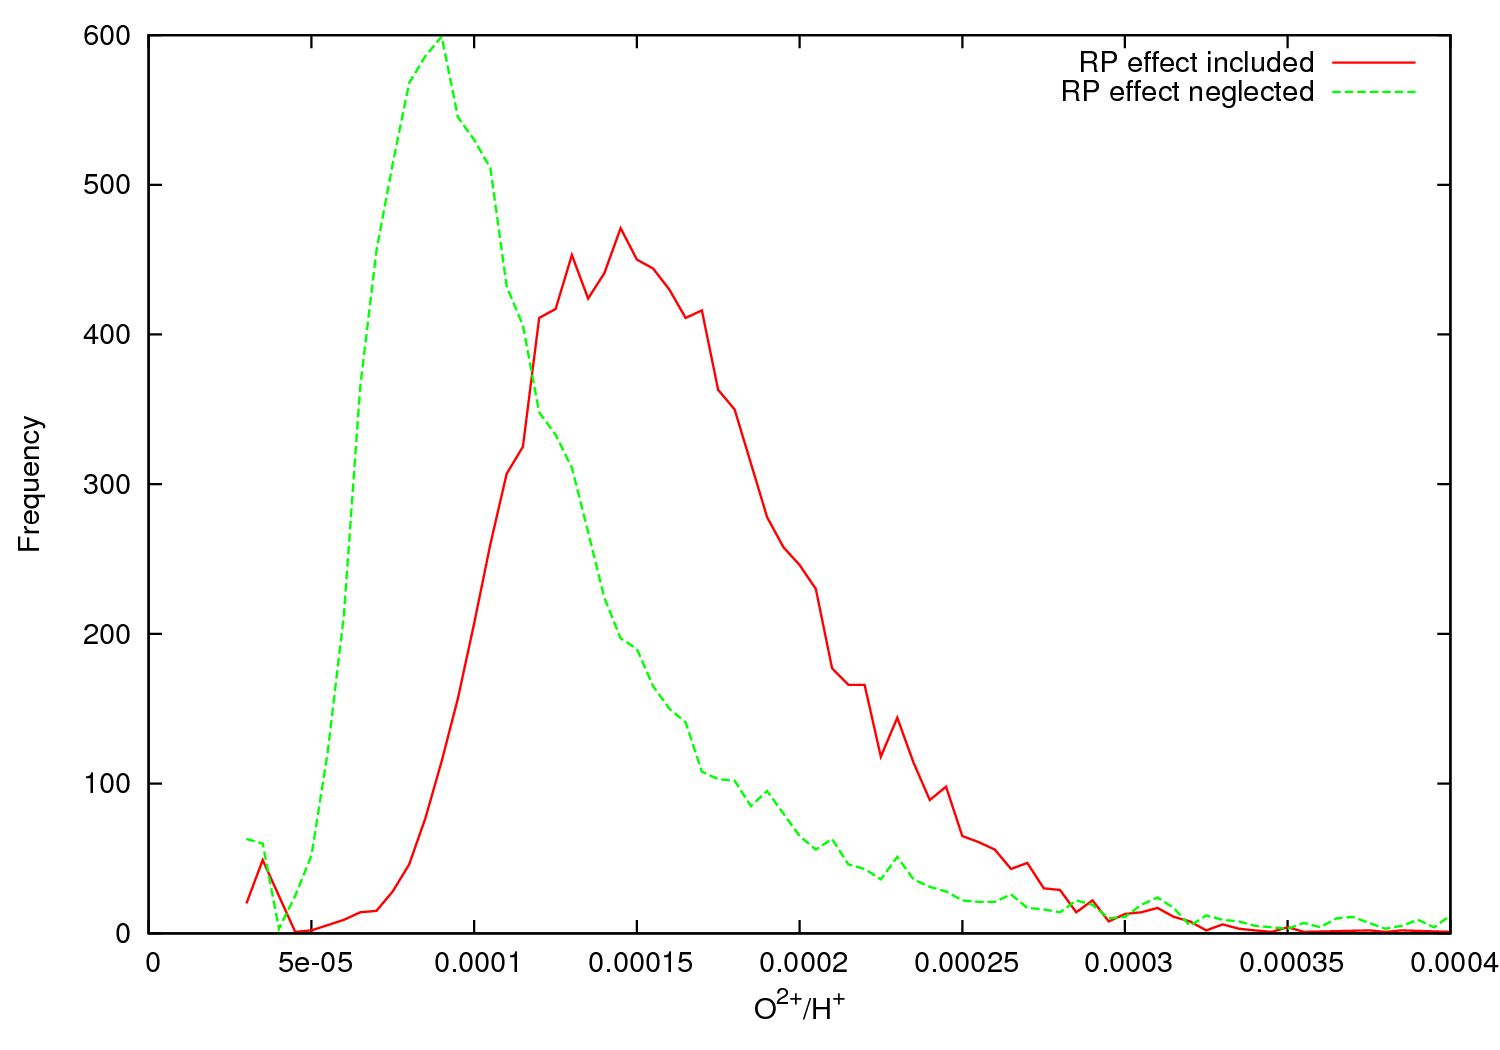
\includegraphics[width=0.48\textwidth]{figures/h1013_rp_abundance.png}
\caption{The RP effect when CEL temperature diagnostic lines are measured with low SNR.  The figure shows a reanalysis of data for the H~{\sc ii} region H1013, showing the RP effect on the derived [O~{\sc iii}] temperature (l) and O$^{2+}$/H$^+$ abundance (r).}
\label{h1013_RP_effect}
\end{figure*}

\section{Interstellar extinction}
\label{extinction}

NEAT allows a robust propagation of uncertainties from line flux measurements into derived quantities.  It is also possible to investigate the effect of uncertainties arising at different stages of the process.  In this section, we consider the effect of the uncertainty in R, the ratio of total to selective extinction given by

\begin{equation}
R = \frac{A(V)}{E(B-V)}
\end{equation}

It is well known that R varies along different sightlines (eg \citet{2004ApJ...616..912V}, \citet{2005ApJ...623..897L}), but estimating its value for particular objects is generally impractical and instead, it is commonly assumed to equal 3.1.  We investigate the effect of an uncertainty in this value by comparing analyses in which R is fixed to be 3.1, and in which R is drawn from a Gaussian distribution with $\mu$=3.1 and $\sigma$=0.15.  For this investigation we used the R-dependent extinction law parametrization of \citet{1989ApJ...345..245C}.  We took the uncertainty as the largest value that we found quoted in the literature for the diffuse ISM \citep{2005ApJ...623..897L}.

We analysed the emission line measurements of NGC 7026 presented by \citet{2005MNRAS.362..424W}, including the line flux uncertainties which were not published in that paper.  We chose this object as it is significantly reddened (c(H$\beta$)=1.0), and has many very well detected lines in its spectrum (142 lines measured, 120 with SNR$>$3 and 65 with SNR$>$10).  This combination should maximise the effect of an uncertainty on R, relative to the effect of the line flux measurement uncertainties.

We find that including the effect of an uncertainty in R has a noticeable effect on the probability distribution of dereddened line fluxes.  However, in the conversion from line fluxes into physical quantities, the statistical uncertainties arising from line flux measurements completely dominate, and the probability distributions are statistically identical whether R is assumed to be fixed or allowed to vary.  This result is shown in Figure~\ref{R_effect}, where we plot the probability distributions for the [Ne~{\sc iii}] 3868{\AA} dereddened line flux, and the abundance derived from it.  The effect on the derived abundance of the assumed uncertainty on R is negligible.

\begin{figure*}
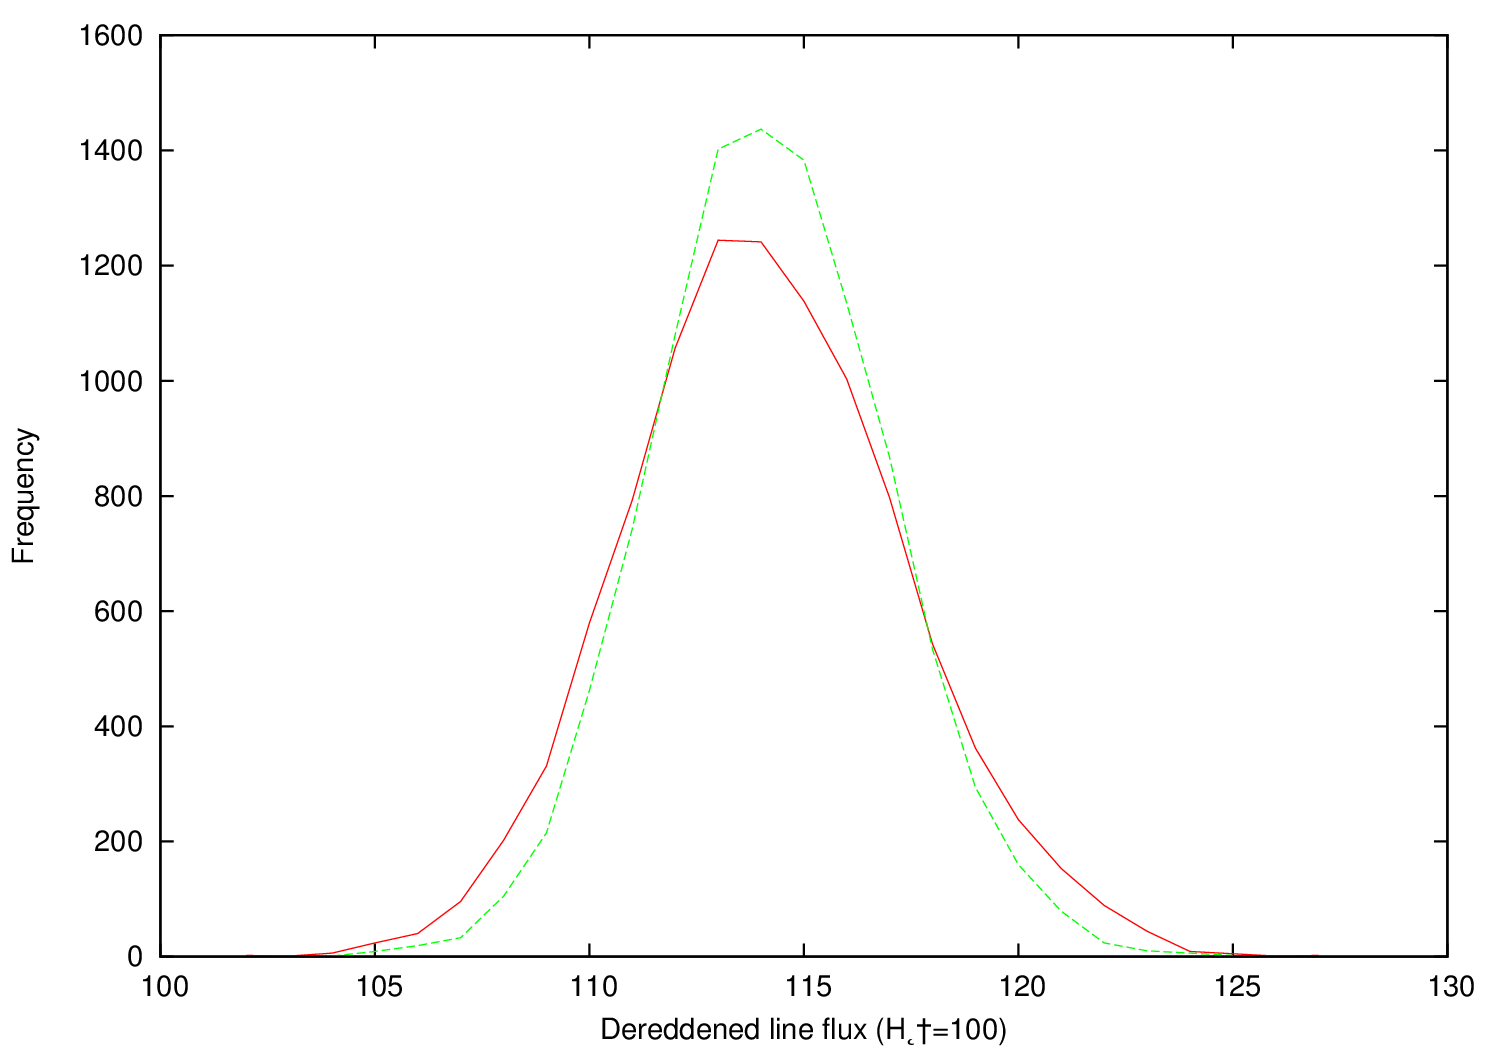
\includegraphics[width=0.48\textwidth]{figures/Reffect_flux.png}
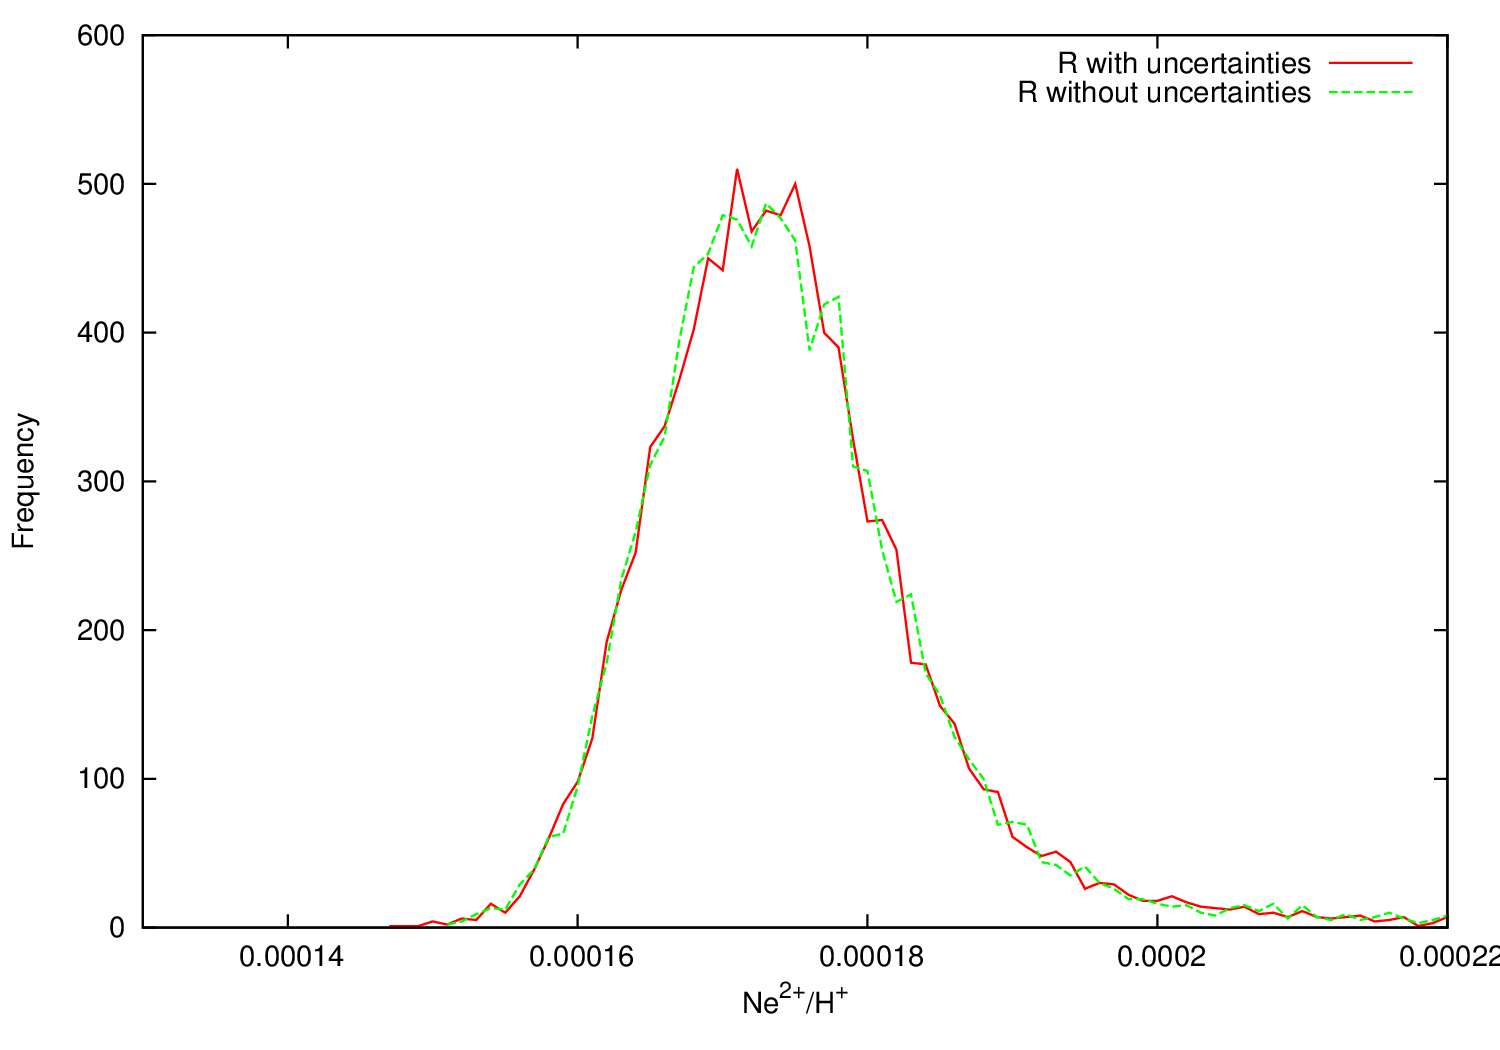
\includegraphics[width=0.48\textwidth]{figures/Reffect_abundance.png}
\caption{The effect of an assumed uncertainty in R, the ratio of selective to total extinction, on the dereddened line flux of the [Ne~{\sc iii}] line at 3868{\AA} (l) and derived Ne$^{2+}$/H$^+$ abundance (r).} 
\label{R_effect}
\end{figure*}

\section{Discussion}

Motivated by the necessity of properly understanding sources of uncertainties in analyses of photoionised nebulae, we have presented a new code for calculating chemical abundances in photoionised nebulae, which also robustly calculates the statistical uncertainties on the abundances determined.  The code is freely available and we welcome bug reports and feature requests.

We have demonstrated that analytic methods of uncertainty propagation rely on assumptions that typically do not hold for real astronomical data, and therefore we have adopted a Monte Carlo approach.  We have shown that the analytic approach does not give a good estimate of the true statistical uncertainties.

We have provided in the code a means for accounting for the well known upward bias in flux measurements of weak lines, and we show that doing so results in significantly improved precision in abundance determinations.  This effect should not be ignored in any analyses of emission line spectra; in almost any data set, the weakest lines will be subject to the effect, and incorrect results will be obtained if the effect is not properly accounted for.  If, as is commonly the case, recombination lines make up the majority of the weak lines, then systematic misunderstandings may arise if the effect is neglected.  However, in the examples that we have analysed, this effect is certainly too small to account for the magnitude of the discrepancy typically found between RL and CEL abundance determinations.

Finally we have shown that possible uncertainties in the value of R have a negligibly small effect on the uncertainties on the final quantities.  This touches upon a further application for the code that we plan to pursue in a forthcoming paper; by varying the {\it systematic} approach being used -- for example, using different atomic data sets, reddening laws or ionisation correction schemes -- we can compare the magnitude of the resulting systematic effects with the true statistical uncertainties, and thus determine realistically which systematic effects are the most important.

\section*{Acknowledgments}

We thank Professor Ian Howarth for useful discussions, Mahesh Mohan for testing an early version of the code, Bruce Duncan for helping us optimise the code, and the organisers of the workshop ``Uncertainties in atomic data and how they propagage in chemical abundances" for providing an extremely fruitful forum for interaction between atomic data providers and users.

\bibliographystyle{mn2e}
\bibliography{NEAT_paper}


\label{lastpage}

\end{document}
